\documentclass{beamer}
\usepackage{graphicx}
\usetheme{metropolis}

\title[BB84]{BB84}
\subtitle{A Quantum Key Distribution Protocol}
\author[Team 37]{Lakshika, Shreya}
\date{July 2020}

\makeatletter
\defbeamertemplate*{frametitle}{myframetitle}{%
    \nointerlineskip
    \begin{beamercolorbox}[%
        wd=\paperwidth,%
        sep=0pt,%
        leftskip=\metropolis@frametitle@padding,
        rightskip=\metropolis@frametitle@padding,
        ]{frametitle}%
        \metropolis@frametitlestrut@start
        \quad\insertframetitle%%%%%%%%%%%%%%%%%%%%%%
        \nolinebreak
        \metropolis@frametitlestrut@end
    \end{beamercolorbox}\par
    \usebeamerfont{framesubtitle}%
    \usebeamercolor[fg]{framesubtitle}%
    \vskip3pt
    \hspace*{-2.5\metropolis@frametitle@padding}%
    \insertframesubtitle
}
%\makeatother
%\setbeamertemplate{frametitle}[myframetitle]

\begin{document}

\begin{frame}
	\titlepage
\end{frame}

\begin{frame}
	\frametitle{Overview}
	 Simulation of BB84 Protocol
\end{frame}


\begin{frame}[standout]
    \begin{columns}
        \column{0.38\linewidth}
            \centering
            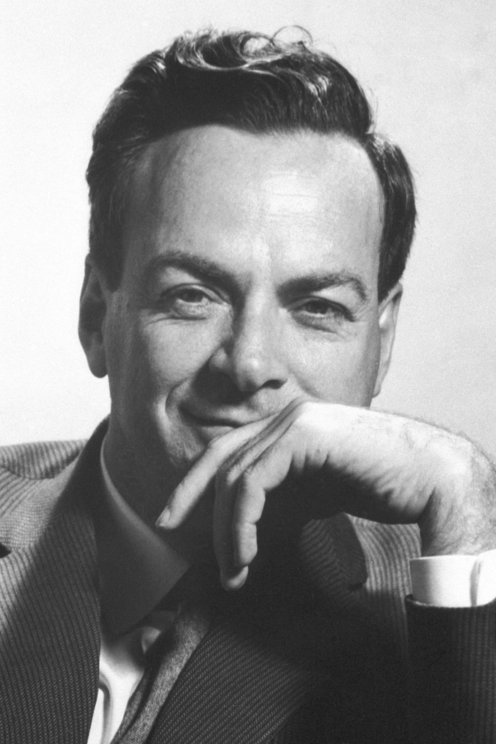
\includegraphics{feynman.jpg}
        \column{0.58\linewidth}
            \emph{Nature isn’t classical, dammit, and if you want to make a simulation of nature, you’d better make it quantum mechanical...}
        \begin{flushright}
            - Richard Feynman
        \end{flushright}
    \end{columns}
\end{frame}


\begin{frame}{Technology Stack}
	\begin{itemize}
		\item Qiskit - An SDK for Quantum Computing
		\item IBM Q - IBM Quantum Experience to access IBM's quantum computers via the cloud
        \item Python Libraries
	\end{itemize}
\end{frame}


\begin{frame}{Quantum Key Distribution}
    \begin{itemize}[<+->]
        \item Key distribution is an important step in Cryptographic protocols
        \item Current protocols assume computational limitations
        \item \begin{itemize}
                \item Quantum Cryptography
                \item Post-Quantum Cryptography
              \end{itemize}
        \item The first QKD protocol by Bennet and Brassard in 1984
     \end{itemize}
\end{frame}


\begin{frame}{The Quantum World}
    \begin{itemize}[<+->]
        \item \textbf{Qubit} - Basic unit of Quantum Information
        \item Bases and Measurement
        \item Communication channels
            \begin{itemize}
                \item A one-way physical Quantum channel
                \item An authenticated two-way classical ideal channel
              \end{itemize}
    \end{itemize}
\end{frame}


\begin{frame}{The BB84 Protocol}
	\framesubtitle{Quantum Phase}
    \begin{itemize}[<+->]
        \item Generation of a random bitstring and bases 
		\item Quantum transmission of encoded bits
		\item Measurement by the receiver
		\item Public comparison of bases and sifting
	\end{itemize}
\end{frame}


\begin{frame}{The BB84 Protocol}
	\framesubtitle{Information Reconciliation}
	The process of cleaning the keys from errors
	\begin{itemize}[<+->]
		\item Error estimation
		\item Low Density Parity Check codes based reconciliation
	\end{itemize}
\end{frame}


\begin{frame}{The BB84 Protocol}
	\framesubtitle{Privacy Amplification}
	\begin{itemize}[<+->]
	    \item Distillation of a highly secret key from a partially secure string by public discussion
		\item Shrinks the possible exposed information over the communication channels to almost zero
		\item 2-Universal hash functions are used
	\end{itemize}
\end{frame}

\begin{frame}{Difficulties faced}
	\begin{itemize}
		\item Getting started with Quantum Computing
        \item In choosing a sub-domain
        \item Unsure about the language and tools to use
		\item Figuring out Information Reconciliation part
	\end{itemize}
\end{frame}


\begin{frame}{Learnings}
	\begin{itemize}
		\item Explored the domain of Quantum Computing
		\item Learnt the basics of Quantum Cryptography
		\item Collecting, reading research papers and trying to understand them
		\item Got introduced to Coding theory
	\end{itemize}
\end{frame}


\end{document}
